\chapter{Python Libraries}

\section{Libraries}
\index{libraries}
A \emph{library} is a collection of pre-written code that provides additional
functionality without requiring you to write everything from scratch. Python
includes many built-in libraries that can be used to perform common tasks such as
mathematical calculations, data handling, and visualization. You'll often find that code you are seeking can be found through an open-source library which already exists.

To use a library, it must first be imported.

\subsection{Importing Libraries}

The simplest way to import a library is using the \mintinline{python}{import} keyword.

\begin{minted}{python}
import math
print(math.sqrt(16))
\end{minted}

In this example, the \mintinline{python}{math} library provides access to mathematical
functions such as square roots.

It is also possible to import specific values or functions from a library.

\begin{minted}{python}
from math import pi
print(pi)
\end{minted}

This allows direct access to \mintinline{python}{pi} without referencing the library name.

\subsection{Summary}

\begin{itemize}
    \item Libraries extend Python's functionality
    \item The \mintinline{python}{import} keyword is used to load libraries
    \item Specific components can be imported directly when needed
\end{itemize}

\section{Matplotlib}
Matplotlib is the most widely used plotting library in Python. It can produce simple charts quickly (line plots, scatter plots, bar charts, histograms) and also supports publication-quality figures with precise control over labels, legends, and layout. We will use it widely throughout this course to visualize data, create simulations for proving formulas, and experiment with datasets. 
\index{matplotlib}\index{creating charts in python|see{matplotlib}}
\subsection{Installing and importing}
If you are working locally, you can install Matplotlib with:
\begin{minted}{bash}
pip install matplotlib
\end{minted}

In most scripts, you will import the plotting interface \texttt{pyplot}:
\begin{minted}{python}
import matplotlib.pyplot as plt
\end{minted}

\subsection{A simple line graph}
A line plot is ideal for showing how a value changes over time or across an ordered variable. Let's create \texttt{line.py} 

\begin{minted}{python}
import matplotlib.pyplot as plt # the matplotlib library, which we will call using plt

# two lists containing values
x = [0, 1, 2, 3, 4, 5]
y = [0, 1, 4, 9, 16, 25]

# a 2d plot, used for line graphs
plt.plot(x, y)
# add a title to our plot
plt.title("A Simple Line Plot")
# add axis labels
plt.xlabel("x")
plt.ylabel("y = x^2")
plt.show() # pops up a new window
\end{minted}
Running \mintinline{bash}|python3 line.py| will open a new \emph{interactive window} in your computer, with the following image:
\begin{figure}[H]
    \centering
    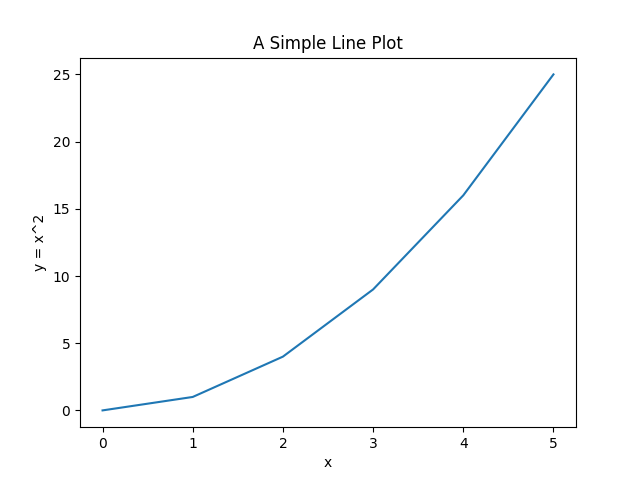
\includegraphics[width=0.6\textwidth]{line.png}
    \caption{The output of line.py.}
    \label{fig:line}
\end{figure}

\subsection{Labels, legends, and grids}
A plot is more useful when it clearly communicates what each element represents. Let's add on to \texttt{line.py} by creating \texttt{lineTwoOutputs.py} and adding labels, a legend, and another set of data. 


\begin{minipage}[t]{0.44\textwidth}
\begin{minted}{python}
import matplotlib.pyplot as plt

x = [0, 1, 2, 3, 4, 5]
y1 = [0, 1, 4, 9, 16, 25]
y2 = [0, 1, 8, 27, 64, 125]

plt.plot(x, y1, label="x^2")
plt.plot(x, y2, label="x^3")

plt.title("Two Functions on One Axes")
plt.xlabel("x")
plt.ylabel("value")
plt.grid(True)
plt.legend()
plt.show()
\end{minted}
\end{minipage}
\begin{minipage}[t]{0.54\textwidth}
\begin{figure}[H]
    \centering
    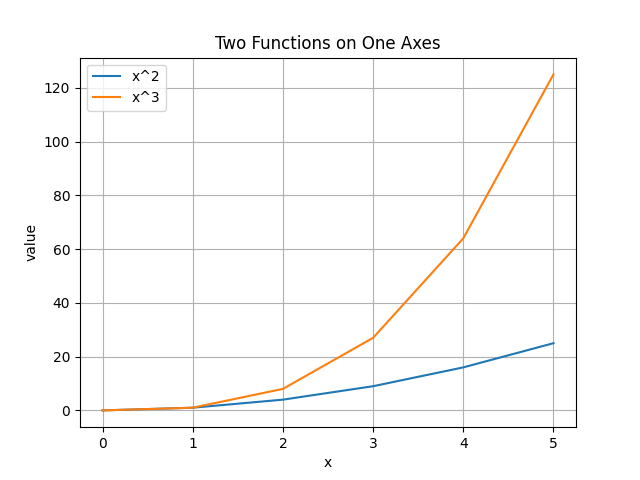
\includegraphics[width=\textwidth]{lineTwoOutputs.png}
    \caption{$y=x^2$ and $y=x^3$ on the same graphed.}
    \label{fig:lineTwoOutputs}
\end{figure}
\end{minipage}
\subsection{Visualizing Relationships with scatter plots}
Scatter plots are excellent for showing how two variables relate (for example, height and weight). 

This very basic scatter plot shows the relationship between studying time and score.

\begin{minipage}[t]{0.44\textwidth}
    
    \begin{minted}{python}
    import matplotlib.pyplot as plt

    hours = [1, 2, 3, 4, 5, 6]
    scores = [55, 60, 66, 72, 78, 85]

    plt.scatter(hours, scores)
    plt.title("Study Time vs. Score")
    plt.xlabel("hours studied")
    plt.ylabel("score")
    plt.show()
    \end{minted}
\end{minipage}
\begin{minipage}[t]{0.54\textwidth}
\begin{figure}[H]
    \centering
    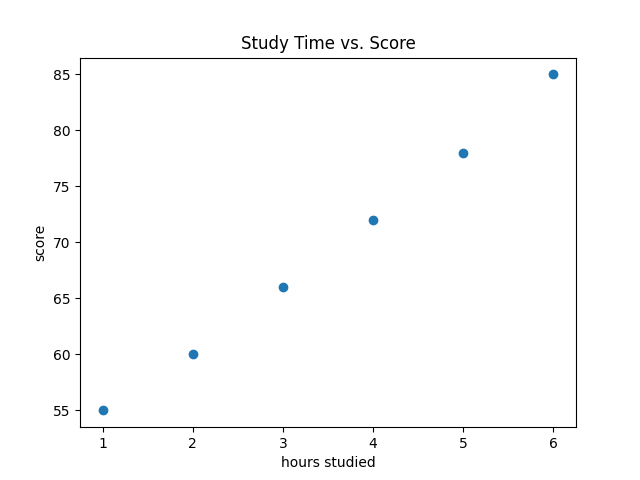
\includegraphics[width=\textwidth]{scatter.png}
    \caption{A scatterplot generated by matplotlib from the given data.}
    \label{fig:scatter}
\end{figure}
\end{minipage}


\subsection{Histograms and Distributions}
A histogram shows how values are distributed and how common different ranges are.

\begin{minipage}[t]{0.44\textwidth}

\begin{minted}{python}
import matplotlib.pyplot as plt
# a set of data, for example maybe these are all test scores
data = [4, 5, 5, 6, 7, 7, 7, 8, 8, 9, 10, 10, 10, 11, 12]

# creates a histogram plot
plt.hist(data, bins=5)
plt.title("Histogram of Values")
plt.xlabel("value")
plt.ylabel("frequency")
plt.show()
\end{minted}
\end{minipage}
\hfill
\begin{minipage}[t]{0.54\textwidth}
    
\begin{figure}[H]
    \centering
    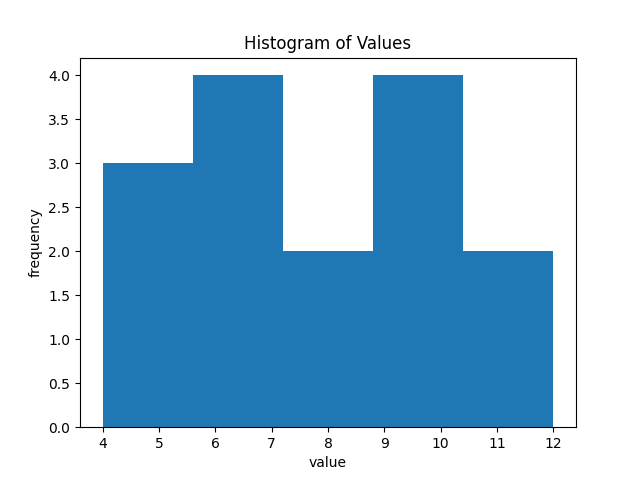
\includegraphics[width=\textwidth]{histogram.png}
    \caption{A histogram of a set of data.}
    \label{fig:histogram}
\end{figure}
        
\end{minipage}

\subsection{The object-oriented approach (recommended)}
Matplotlib has two main styles:
\begin{itemize}
  \item \textbf{State-based} (using \texttt{plt.plot}, \texttt{plt.title}, \dots): quick and convenient.
  \item \textbf{Object-oriented} (creating a \texttt{Figure} and \texttt{Axes}): more explicit and easier to scale.
\end{itemize}

For multi-plot layouts or different analysis of datasets, prefer the object-oriented approach:
    
\begin{minted}{python}
import matplotlib.pyplot as plt

x = [0, 1, 2, 3, 4, 5]
y1 = [0, 1, 4, 9, 16, 25]
y2 = [0, 1, 8, 27, 64, 125]

# two figures, side by side. axes becomes an indexable list
fig, axes = plt.subplots(nrows=1, ncols=2)

axes[0].plot(x, y1)
axes[0].set_title("x^2")
axes[0].set_xlabel("x")
axes[0].set_ylabel("value")

axes[1].plot(x, y2)
axes[1].set_title("x^3")
axes[1].set_xlabel("x")
axes[1].set_ylabel("value")

fig.suptitle("Two Subplots")
fig.tight_layout()
plt.show()
\end{minted}
\begin{figure}[H]
    \centering
    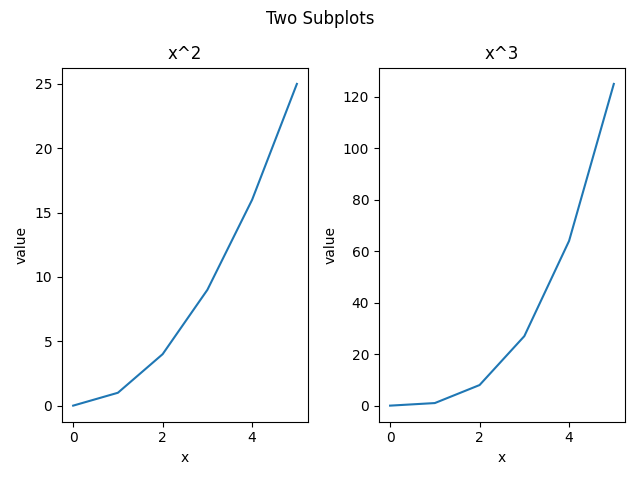
\includegraphics[width=\textwidth]{lineOOP.png}
    \caption{The two plots, generated side by side.}
    \label{fig:lineOOP}
\end{figure}
